\documentclass[a4paper]{article}

\usepackage[paper=a4paper, left=1.5cm, right=1.5cm, bottom=1.5cm, top=2.5cm]{geometry}
\usepackage[spanish,activeacute]{babel}
\usepackage[utf8]{inputenc}
\usepackage{amsthm}
\usepackage{amsmath}
\usepackage{amsfonts}
\usepackage{amssymb}
\usepackage{alltt}
\usepackage{graphicx} %Para incluir el logo de la UBA
\usepackage{caratula} %Para armar el cuadro de integrantes
\usepackage{multirow} %Para poder poner varias lineas juntas sin divisiones en una tabla
\usepackage{algorithm2e}
\usepackage{algpseudocode}
\usepackage{scrextend}
\usepackage{blindtext}
\usepackage{colortbl}
\usepackage{color}

%Cosas para escribir codigo fuente
%Fuente: http://en.wikibooks.org/wiki/LaTeX/Source_Code_Listings
\usepackage{listings}
\usepackage{color}

\setcounter{secnumdepth}{5}

\definecolor{mygreen}{rgb}{0,0.6,0}
\definecolor{mygray}{rgb}{0.5,0.5,0.5}
\definecolor{myorange}{rgb}{1,0.4,0.2}
\definecolor{myblue}{rgb}{0,0,0.65}

%Configuracion para los listings
\lstset{ %
  backgroundcolor=\color{white},   % choose the background color; you must add \usepackage{color} or \usepackage{xcolor}
  basicstyle=\small,        % the size of the fonts that are used for the code
  breakatwhitespace=false,         % sets if automatic breaks should only happen at whitespace
  breaklines=true,                 % sets automatic line breaking
  captionpos=b,                    % sets the caption-position to bottom
  commentstyle=\color{mygreen},    % comment style
  deletekeywords={...},            % if you want to delete keywords from the given language
  escapeinside={\%*}{*)},          % if you want to add LaTeX within your code
  extendedchars=true,              % lets you use non-ASCII characters; for 8-bits encodings only, does not work with UTF-8
  frame=single,                    % adds a frame around the code
  keywordstyle=\color{myblue},       % keyword style
  language=Octave,                 % the language of the code
  morekeywords={*,...},            % if you want to add more keywords to the set
  numbers=left,                    % where to put the line-numbers; possible values are (none, left, right)
  numbersep=5pt,                   % how far the line-numbers are from the code
  numberstyle=\tiny\color{mygray}, % the style that is used for the line-numbers
  rulecolor=\color{black},         % if not set, the frame-color may be changed on line-breaks within not-black text (e.g. comments (green here))
  showspaces=false,                % show spaces everywhere adding particular underscores; it overrides 'showstringspaces'
  showstringspaces=false,          % underline spaces within strings only
  showtabs=false,                  % show tabs within strings adding particular underscores
  stepnumber=1,                    % the step between two line-numbers. If it's 1, each line will be numbered
  stringstyle=\color{myorange},     % string literal style
  tabsize=2,                       % sets default tabsize to 2 spaces
  title=\lstname                   % show the filename of files included with \lstinputlisting; also try caption instead of title
}

\renewcommand{\lstlistingname}{C\'{o}digo}

\lstset{language=C++,caption={Descriptive Caption Text},label=DescriptiveLabel}
\setlength\parindent{0pt}

%\topmargin = -1cm
%\textheight = 24cm 

\begin{document}


\integrante{Sclar, Melanie}{551/12}{melaniesclar@gmail.com}
\integrante{Zylber, Ariel}{530/12}{arielzylber@gmail.com}

\def\Materia{Final de Organizaci\'on del Computador II}
\def\Fecha{Muy pronto}

%----- CARATULA -----%

\thispagestyle{empty}

\begin{center}
	
\includegraphics[scale = 0.25]{logo_uba.jpg}
\end{center}

\vspace{5mm}

\begin{center}
	{\textbf{\large UNIVERSIDAD DE BUENOS AIRES}}\\[1.5em]
	{\textbf{\large Departamento de Computaci\'{o}n}}\\[1.5em]
    {\textbf{\large Facultad de Ciencias Exactas y Naturales}}\\
    \vspace{35mm}
    {\LARGE\textbf{\Materia}}\\[1em]    
    \vspace{15mm}
    {\Large \textbf{\Titulo}}\\[1em]
    \vspace{15mm}
    {\textbf{\Large \Fecha}}\\
    \vspace{15mm}
    \textbf{\tablaints}
\end{center}

\newtheorem{teo}{Teorema}[section]
\newtheorem{propo}{Proposici\'{o}n}[section]
\newtheorem{lema}{Lema}[section]
\newtheorem{coro}{Corolario}[section]
\newtheorem{defi}{Definici\'{o}n}[section]

\newpage
\setcounter{page}{1}
\pagenumbering{arabic}
\pagestyle{plain}

\newpage


\newcommand{\Asig}{\ensuremath{\leftarrow}}
\newcommand{\AndY}{\ensuremath{\wedge}}
\newcommand{\Or}{\ensuremath{\vee}}
\newcommand{\Not}{\ensuremath{\neg}}
\newcommand{\NotEq}{\ensuremath{\neq}}
\newcommand{\MayorIg}{\ensuremath{\geq}}
\newcommand{\tabu}{\hspace*{0.7cm}}
\newcommand{\ctabu}{\hspace*{0.8cm}}
\newcommand{\htabu}{\hspace*{0.35cm}}
\newcommand{\moduloNombre}[1]{\textbf{#1}}

\section{Objetivo del trabajo}

El objetivo del trabajo es resolver la ecuación de Biocalor de Pennes 
utilizando el método de Jacobi para calcular la temperatura en cada 
sección de un tejido a cada instante de tiempo. Esto se enmarca dentro 
de los proyectos del Laboratorio de Sistemas Complejos (DC-UBA), pues 
el LSC aplicará nuestro trabajo para agilizar el cálculo de una sección 
de su modelo para identificar la temperatura y posición óptimas en las 
que aplicar un tratamiento para reducir los tumores cancerígenos. A 
grandes rasgos, los tratamientos ultilizados consiste en colocar dos electrodos (un 
ánodo y un cátodo) en puntos específicos de la piel del paciente 
cercanos al tumor y lograr la destrucción del tejido cancerígeno 
debido a cambios de pH, aumento de permeabilidad irreversible en la 
membrana plasmática o aumento en la absorción del quimioterápico, 
entre otros. Como efecto secundario del tratamiento se produce un 
aumento de temperatura en el tejido. Nosotros desarrollaremos un 
modelo para simular calentamiento del tejido y así poder estudiar 
que consecuencias trae al paciente. Gráficamente,\\

\begin{figure}[!htbp]
  \centering
	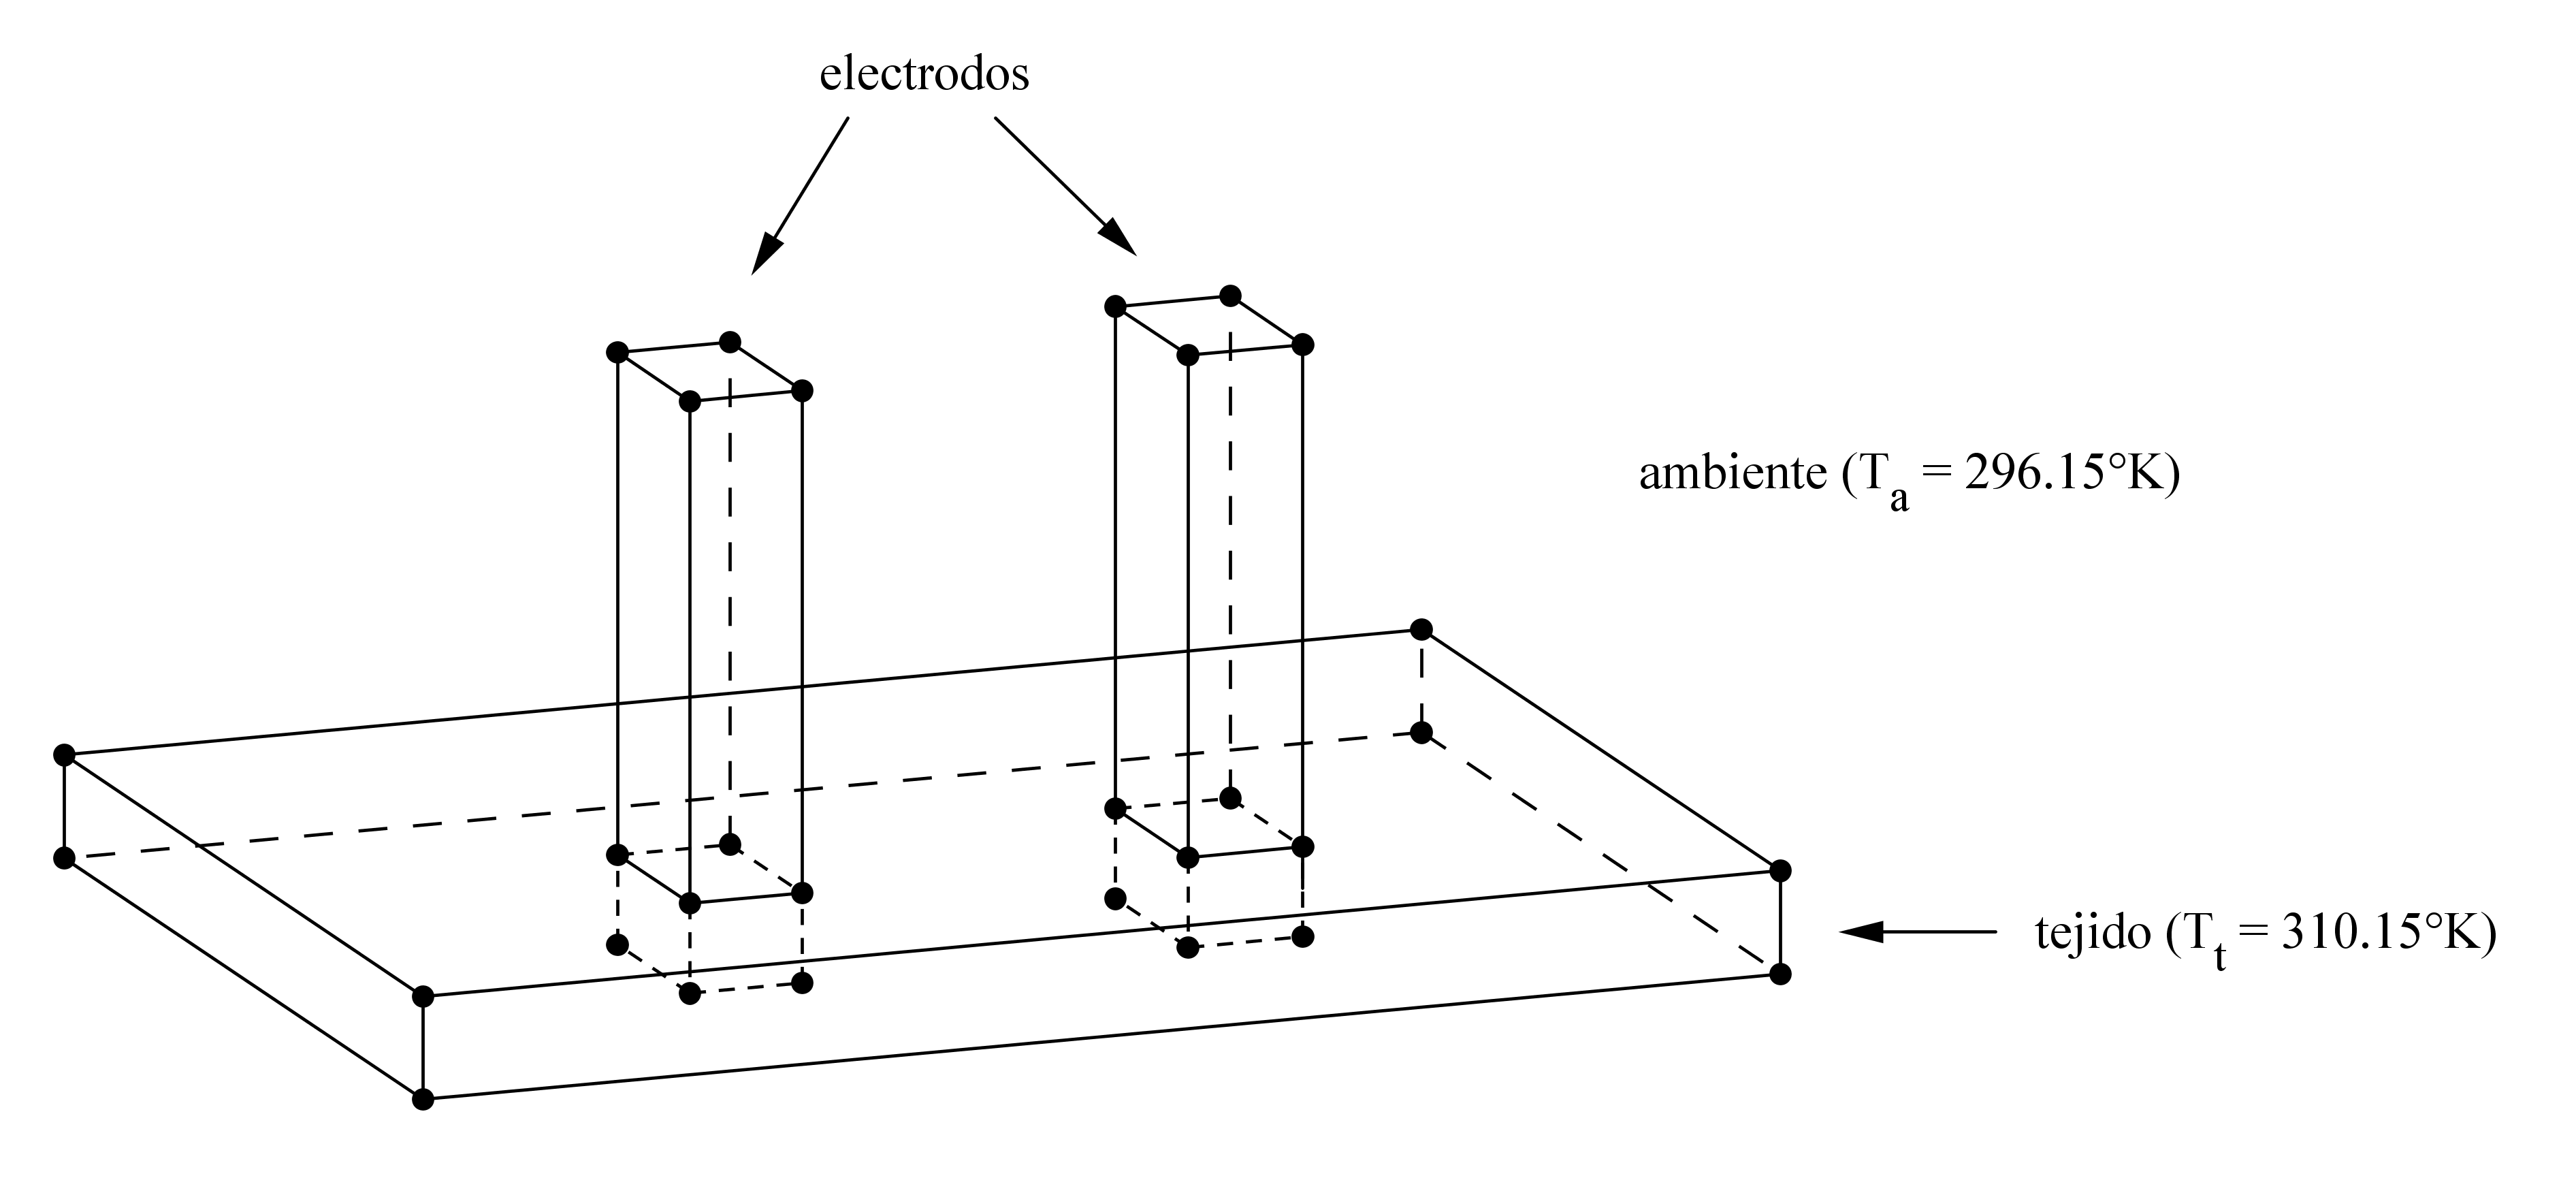
\includegraphics[scale = 0.18]{tejido-anotado.png}
  \caption{Representación gráfica del tratamiento para el tumor}
\end{figure}

Además de resolver la ecuación de Pennes, se resolverá la ecuación
de Laplace para calcular el potencial eléctrico del tejido (que es uno de los parámetros
de la ecuación de Pennes). Una explicación detallada de su cálculo se podrá ver más adelante.\\

Como la resolución de estas ecuaciones ocupa una parte no despreciable 
del cómputo de sus algoritmos completos, lo implementamos en C plano y en ASM con SIMD y 
compararemos los tiempos de ejecución obtenidos con cada una (compilando con gcc e icc). Creemos que 
utilizar SIMD podría ser muy provechoso en este problema, ya que muchas 
de las operaciones de matrices que efectuaremos son paralelizables y 
esperamos ver una significante reducción en el tiempo de ejecución del 
algoritmo. Notar que se aprovechará la estructura particular del problema para optimizar al máximo la
resolución: el programa resultante es más complejo pero esto hace que se reduzca la complejidad
temporal del programa en varios órdenes.\\

Como todos los cálculos son con números de punto flotante con doble 
precisión, utilizaremos los registros YMM (cuya longitud es el doble que la de los
registros XMM vistos en la materia) para poder paralelizar el cálculo de 4 números en vez de sólo 2.\\

Cabe destacar que el LSC no tenía implementación alguna de esto que vamos
a resolver, por lo que parte del alcance del trabajo fue dar un programa
en C que resuelva correctamente el problema. La comprobación de que los resultados 
fue no trivial, e incluyó consultas a diversos integrantes del LSC para
realizar un análisis cuantitativo y cualitativo de los resultados. Una explicación del
análisis realizado y sus resultados gráficos se mostrará al final del trabajo.

\newpage
\section{Distribuci\'on de la temperatura: obtención del sistema a resolver}

A continuación partiremos de la ecuación de Biocalor de Pennes y despejaremos
el sistema de ecuaciones a resolver. Cada punto del tejido tiene una 
ecuación que describe la evolución de su temperatura: la mayoría de los puntos
se rigen por las ecuaciones obtenidas en la sección 2.1, mientras que los bordes
tienen sus particularidades que se describen en la sección 2.2. 
Llamamos $bordes$ tanto a los bordes exteriores del recinto
(los bordes de la matriz) como a los puntos donde se aplican los electrodos.
Las ecuaciones nos fueron ya dadas por el LSC, y nosotros únicamente las 
comprobamos, hicimos las correcciones necesarias e implementamos en C y ASM.

\subsection{Temperatura en todo el tejido salvo los bordes}

Partimos de la ecuación de Biocalor de Pennes, 
$$\nabla \cdot (k \nabla T) - w_b C_b \rho_b (T-T_a) + q''' + \sigma |\nabla \varphi|^2 = \rho \ C_\rho \ \frac{\partial T}{\partial t}$$

Donde $\sigma$ es la conductividad eléctrica, $\phi$ es el potencial eléctrico, $k$ es la conductividad térmica, $T_a$ es la temperatura arterial, $w_b$ es la blood perfusion rate, $C_b$ es la capacidad calorífica de la sangre, $\rho_b$ es la densidad de la sangre, $q'''$ es la generación de calor metabólico, $\rho$ es la densidad del tejido y $C_\rho$ es la capacidad calorífica del tejido.\\

Para nuestro modelo, hay varias constantes que suponemos conocidas, en los siguientes valores:

$C_\rho= 3680$, $\rho= 1039$, $q'''= 10437$, $C_b= 3840$, $\rho_b= 1060$, $w_b=7.15 \ 10^{-3}$, $T_a = 310.15^\circ K$ \\

$k$, $\sigma$ y $\varphi$ son campos escalares variables. Sin embargo, a la hora de realizar los cálculos tomaremos los siguientes valores para las funciones,
como fue indicado por Emmanuel Luján. 

$k(x,y)=0.565$ \\
$\sigma(x,y)=0.75$ \\

Para calcular $\varphi$ supondremos dado un ánodo en la posición $(x_a, y_a)$ con potencial eléctrico 
constante $q_a$ y un cátodo en la posición $(x_c, y_c)$ con potencial eléctrico 
constante $q_c$. Luego obtenemos como se extiende la $\varphi$ a todo el recinto 
resolviendo la ecuación de Laplace dados los puntos del ánodo y cátodo fijos y 
condición de borde de flujo cero. Para más detalles sobre como calcular esto ver apéndice B.
\textbf{La resolución de la ecuación de Laplace también formará parte de nuestro trabajo de implementación.}\\

Notar que en estos valores particulares los campos son constantes en el tiempo pero al realizar la discretización del problema no lo supondremos constante que sino lo haremos en la versión general donde sus valores podrían depender del tiempo.

Entonces, los únicos valores desconocidos para nosotros son los $T_n(i,j)$, es decir, el valor de la temperatura en el tiempo $n$ (ya discretizado) en cada lugar del espacio $(i,j)$.
Utilizaremos las discretizaciones tal y como nos fueron indicadas: el término temporal por diferencias adelantadas, los términos espaciales por diferencias centradas. \\

A continuación calcularemos el término $\nabla \cdot (k \nabla T)$:
\begin{equation} \label{eq:nablaT}
\begin{split}
\nabla \cdot (k \nabla T) & = \nabla \cdot k \bigg(\frac{\partial T}{\partial x}, \frac{\partial T}{\partial y}\bigg) \\
& = \frac{\partial}{\partial x} \bigg(k \frac{\partial T}{\partial x}\bigg) + \frac{\partial}{\partial y} \bigg(k \frac{\partial T}{\partial y}\bigg) \\
& = \frac{\partial k}{\partial x} \cdot \frac{\partial T}{\partial x} + k \cdot \frac{\partial^2 T}{\partial x^2} + \frac{\partial k}{\partial y} \cdot \frac{\partial T}{\partial y} + k \cdot \frac{\partial^2 T}{\partial y^2} \\
 & = \frac{\partial k}{\partial x} \cdot \frac{\partial T}{\partial x} + \frac{\partial k}{\partial y} \cdot \frac{\partial T}{\partial y} + k \cdot \frac{\partial^2 T}{\partial x^2} + k \cdot \frac{\partial^2 T}{\partial y^2}
\end{split}
\end{equation}

Notar que si $k$ es constante, $\frac{\partial k}{\partial x} = \frac{\partial k}{\partial y} = \frac{\partial k}{\partial t} = 0$ y por lo tanto, obtenemos $\nabla \cdot (k \nabla T) = k \cdot \frac{\partial^2 T}{\partial x^2} + k \cdot \frac{\partial^2 T}{\partial y^2} + k \cdot \frac{\partial^2 T}{\partial t^2}$ \\
Sin embargo, a priori no sabemos que nuestro modelo de aplicación será con $k$ constante así que deberemos calcular sus derivadas. Mostramos cómo se calculan todas las derivadas respecto de $T$ con sus discretizaciones, y para $k$ será análogo.

\begin{equation*}
\begin{split}
\frac{\partial T}{\partial x} & \approx \frac{T_{n+1}(i+1,j) - T_{n+1}(i-1,j)}{\Delta x_i + \Delta x_{i+1}} \\
\frac{\partial T}{\partial y} & \approx \frac{T_{n+1}(i,j+1) - T_{n+1}(i,j-1)}{\Delta y_j + \Delta y_{j+1}} \\
\frac{\partial^2 T}{\partial x^2} & \approx \frac{2 T_{n+1}(i+1,j)}{\Delta x_i (\Delta x_i + \Delta x_{i-1})} - \frac{2 T_{n+1}(i,j)}{\Delta x_i \Delta x_{i-1}} + \frac{2 T_{n+1}(i-1,j)}{\Delta x_{i-1} (\Delta x_i + \Delta x_{i-1})} \\
\frac{\partial^2 T}{\partial y^2} & \approx \frac{2 T_{n+1}(i,j+1)}{\Delta y_j (\Delta y_j + \Delta y_{j-1})} - \frac{2 T_{n+1}(i,j)}{\Delta y_j \Delta y_{j-1}} + \frac{2 T_{n+1}(i,j-1)}{\Delta y_{j-1} (\Delta y_j + \Delta y_{j-1})} \\
\frac{\partial T}{\partial t} & \approx \frac{T_{n+1}(i,j) - T_n(i,j)}{\Delta t_n}
\end{split}
\end{equation*}

Como podemos asumir que $\Delta x_i = \Delta x_j = \Delta x$ y $\Delta y_i = \Delta y_j = \Delta y$ para todo $i$, $j$, las ecuaciones quedan así:
\begin{equation} \label{eq:derivadas}
\begin{split}
\frac{\partial T}{\partial x} & \approx \frac{T_{n+1}(i+1,j) - T_{n+1}(i-1,j)}{2\Delta x}  \\
\frac{\partial T}{\partial y} & \approx \frac{T_{n+1}(i,j+1) - T_{n+1}(i,j-1)}{2\Delta y} \\
\frac{\partial^2 T}{\partial x^2} & \approx \frac{T_{n+1}(i+1,j)}{(\Delta x)^2} - \frac{2 T_{n+1}(i,j)}{(\Delta x)^2} + \frac{T_{n+1}(i-1,j)}{(\Delta x)^2} \\
\frac{\partial^2 T}{\partial y^2} & \approx \frac{T_{n+1}(i,j+1)}{(\Delta y)^2} - \frac{2 T_{n+1}(i,j)}{(\Delta y)^2} + \frac{T_{n+1}(i,j-1)}{(\Delta y)^2} \\
\frac{\partial T}{\partial t} & \approx \frac{T_{n+1}(i,j) - T_n(i,j)}{\Delta t}
\end{split}
\end{equation}

Aplicando todo esto a la ecuación del Biocalor de Pennes, despejamos los coeficientes de $T_n$ en función de los de $T_{n+1}$, para obtener un sistema de ecuaciones a resolver con Jacobi. Tomemos la ecuación del Biocalor de Pennes:
$$\nabla \cdot (k \nabla T) - w_b C_b \rho_b (T-T_a) + q''' + \sigma |\nabla \varphi|^2 = \rho \ C_\rho \ \frac{\partial T}{\partial t}$$

Reemplazando con lo obtenido en (\ref{eq:nablaT}),
$$ \frac{\partial k}{\partial x} \cdot \frac{\partial T}{\partial x} + \frac{\partial k}{\partial y} \cdot \frac{\partial T}{\partial y} + k \cdot \frac{\partial^2 T}{\partial x^2} + k \cdot \frac{\partial^2 T}{\partial y^2} - w_b C_b \rho_b (T-T_a) + q''' + \sigma |\nabla \varphi|^2 = \rho \ C_\rho \ \frac{\partial T}{\partial t}$$

Luego, aproximamos las derivadas como definimos en (\ref{eq:derivadas}):\\
\begin{equation*}
\begin{aligned}
\rho \ C_\rho \ \frac{T_{n+1}(i,j) - T_n(i,j)}{\Delta t} &= \frac{\partial k}{\partial x} \cdot \frac{T_{n+1}(i+1,j) - T_{n+1}(i-1,j)}{2\Delta x} \\ & \ \ \ \ \ \ \  + \frac{\partial k}{\partial y} \cdot \frac{T_{n+1}(i,j+1) - T_{n+1}(i,j-1)}{2\Delta y} \\ & \ \ \ \ \ \ \ + k \cdot \bigg(\frac{T_{n+1}(i+1,j)}{(\Delta x)^2} - \frac{2 T_{n+1}(i,j)}{(\Delta x)^2} + \frac{T_{n+1}(i-1,j)}{(\Delta x)^2}\bigg) \\ & \ \ \ \ \ \ \  + k \cdot \bigg(\frac{T_{n+1}(i,j+1)}{(\Delta y)^2} - \frac{2 T_{n+1}(i,j)}{(\Delta y)^2} + \frac{T_{n+1}(i,j-1)}{(\Delta y)^2}\bigg) \\ & \ \ \ \ \ \ \  -  w_b C_b \rho_b (T_{n+1}(i,j)-T_a) + q''' + \sigma |\nabla \varphi|^2\\
\end{aligned}
\end{equation*}

\bigskip
Ahora sí, despejemos $T_n$ en función de los de $T_{n+1}$. Para abreviar, sea $TInd = w_b C_b \rho_b T_a + q''' + \sigma |\nabla \varphi|^2$. \\

\begin{equation*}
\begin{aligned}
- T_n(i,j) \frac{\rho \ C_\rho}{\Delta t} - TInd(i,j) &= T_{n+1}(i+1,j) \cdot \bigg(\frac{\partial k}{\partial x} \cdot \frac{1}{2\Delta x} +  k \cdot\frac{1}{(\Delta x)^2}\bigg) \\ & \ \ \ \ \ \ \ + T_{n+1}(i-1,j) \cdot \bigg(-\frac{\partial k}{\partial x} \cdot \frac{1}{2\Delta x} + k \cdot\frac{1}{(\Delta x)^2}\bigg) \\ & \ \ \ \ \ \ \ + T_{n+1}(i,j) \cdot \bigg(-\frac{2k}{(\Delta x)^2} -\frac{2k}{(\Delta y)^2} - w_b C_b \rho_b - \rho \ C_\rho \ \frac{1}{\Delta t}\bigg) \\ & \ \ \ \ \ \ \ + T_{n+1}(i,j+1) \cdot \bigg(\frac{\partial k}{\partial y} \cdot \frac{1}{2\Delta y} + k \cdot\frac{1}{(\Delta y)^2}\bigg) \\ & \ \ \ \ \ \ \  + T_{n+1}(i,j-1) \cdot \bigg(-\frac{\partial k}{\partial y} \cdot \frac{1}{2\Delta y} + k \cdot\frac{1}{(\Delta y)^2}\bigg)
\end{aligned}
\end{equation*}

Con estas ecuaciones nos quedará un sistema a resolver, pero antes de plantearlo debemos explicitar cuáles serán las condiciones de borde en este problema, ya que las ecuaciones antes dichas no valen en el borde exterior ni alrededor del ánodo y cátodo.

\subsection{Temperatura en los bordes}

\subsubsection{Temperatura en bordes exteriores}
La condición de borde del sistema es de flujo cero, es decir $q \cdot \hat{n} = 0$ donde $\hat{n}$ es el vector unitario normal al borde del recinto. Esto quiere decir que $-K \nabla T \cdot \hat{n} = 0$, dividiendo por $-K$ queda $\nabla T \cdot \hat{n} = 0$. Esto se interpreta como que en el borde la derivada en la dirección hacia adentro es nula. Al discretizar, esto se traduce en que la diferencia entre la temperatura en un punto del borde y su inmediato vecino interno es nula, es decir que son iguales. Más formalmente, asumiremos que:
\begin{equation*}
\begin{aligned}
T_{n+1}(0,j) & = T_{n+1}(1,j) \\ 
T_{n+1}(i,0) & = T_{n+1}(i,1) \\
T_{n+1}(i,max_j) & = T_{n+1}(i,max_j-1) \\ 
T_{n+1}(max_i,j) & = T_{n+1}(max_i-1,j)
\end{aligned}
\end{equation*}

\subsubsection{Temperatura en los puntos del tejido donde se aplican los electrodos}
Además, en el borde de los electrodos (ánodo y cátodo) el cálculo de la temperatura es diferente. Los detalles de su cálculo se pueden ver en el Apéndice A. Siendo $(i,j)$ la aproximación del borde del electrodo,

$$T_{n+1}(i,j) = \frac{r}{4(r-1)} \cdot \big( T_{n+1}(i+1,j) + T_{n+1}(i,j+1) + T_{n+1}(i-1,j) + T_{n+1}(i,j-1)\big) - \frac{T_{aire}}{r-1}$$

Donde $r = \frac{k}{\Delta x \cdot h}$, $h = 10 \frac{W}{m^2 K}$ y $T_{aire} = 296 ^\circ K$.\\ 

En nuestro trabajo, las posiciones de los electrodos serán parte del input del programa.

\subsection{Planteo del sistema y resolución}

Habiendo hallado todas las ecuaciones que relacionan $T_n$ con $T_{n+1}$, 
podemos escribir un sistema a resolver de la forma $$A \cdot T_{n+1} = B$$ donde 
$B = -\frac{\rho \cdot C_\rho}{\Delta t} \cdot T_n - TInd$ y 
despejar $T_{n+1}$ utilizando Jacobi. Consideramos a $A$ como la matriz 
cuadrada de lado $max_i \cdot max_j$ donde cada fila corresponde a 
una posición $(i, j)$ de la discretización de modo que en la fila de la 
posición $(i, j)$ tendremos los coeficientes de la ecuación correspondiente 
a $T_n(i,j)$ para cada posición de la grilla. Notemos que luego de hallar $T_n$, 
la única incógnita del sistema es en efecto $T_{n+1}$ y en efecto se puede 
aplicar Jacobi usualmente.\\

Notemos que la matriz $A$ es esparsa, pues en cada fila los coeficientes 
que podrían ser no nulos corresponden a las posiciones del punto en 
cuestión y sus vecinos. Con esto conseguiremos reducir mucho el tiempo 
de cómputo en todas las implementaciones. Esto también implicó un crecimiento
en la complejidad del código a paralelizar, pues ya no es una simple resolución
de sistema de ecuaciones sino que hay que tener sumo cuidado en respetar
los índices indicados como no nulos. \\

Gráficamente, si $A$ fuera una matriz de $6 \times 6$ los únicos lugares que pueden
ser no nulos son los que se muestran en gris en la imagen. Para la fila 
correspondiente a $(i,j)$, los únicos elementos no nulos pueden ser $(i, j-1)$, 
$(i,j+1)$ (que se verán a la izquierda y a la derecha de $(i,j)$ respectivamente), 
$(i-1, j)$ e $(i+1,j)$ (que al estar una fila arriba o abajo de $(i,j)$, 
en el gráfico se verán $max_j = 6$ lugares para la izquierda o para la derecha de él). 

\begin{table}[!htbp]
\centering
\label{matriz_a}
\begin{tabular}{|l|l|l|l|l|l|l|l|l|l|l|l|l|l|l|l|l|l|l|l|l|l|l|l|l|l|l|l|l|l|l|l|l|l|l|l|}
\hline
 & & & & & & & & & & & & & & & & & & & & & & & & & & & & & & & & & & & \\ \hline 
 & & & & & & & & & & & & & & & & & & & & & & & & & & & & & & & & & & & \\ \hline 
 & & & & & & & & & & & & & & & & & & & & & & & & & & & & & & & & & & & \\ \hline 
 & & & & & & & & & & & & & & & & & & & & & & & & & & & & & & & & & & & \\ \hline 
 & & & & & & & & & & & & & & & & & & & & & & & & & & & & & & & & & & & \\ \hline 
 & & & & & & & & & & & & & & & & & & & & & & & & & & & & & & & & & & & \\ \hline 
 & & & & & & & & & & & & & & & & & & & & & & & & & & & & & & & & & & & \\ \hline 
 & \cellcolor{mygray} & & & & & \cellcolor{mygray} & \cellcolor{mygray} & \cellcolor{mygray} & & & & & \cellcolor{mygray} & & & & & & & & & & & & & & & & & & & & & & \\ \hline 
 & & \cellcolor{mygray} & & & & & \cellcolor{mygray} & \cellcolor{mygray} & \cellcolor{mygray} & & & & & \cellcolor{mygray} & & & & & & & & & & & & & & & & & & & & & \\ \hline 
 & & & \cellcolor{mygray} & & & & & \cellcolor{mygray} & \cellcolor{mygray} & \cellcolor{mygray} & & & & & \cellcolor{mygray} & & & & & & & & & & & & & & & & & & & & \\ \hline 
 & & & & \cellcolor{mygray} & & & & & \cellcolor{mygray} & \cellcolor{mygray} & \cellcolor{mygray} & & & & & \cellcolor{mygray} & & & & & & & & & & & & & & & & & & & \\ \hline 
 & & & & & & & & & & & & & & & & & & & & & & & & & & & & & & & & & & & \\ \hline 
 & & & & & & & & & & & & & & & & & & & & & & & & & & & & & & & & & & & \\ \hline 
 & & & & & & & \cellcolor{mygray} & & & & & \cellcolor{mygray} & \cellcolor{mygray} & \cellcolor{mygray} & & & & & \cellcolor{mygray} & & & & & & & & & & & & & & & & \\ \hline 
 & & & & & & & & \cellcolor{mygray} & & & & & \cellcolor{mygray} & \cellcolor{mygray} & \cellcolor{mygray} & & & & & \cellcolor{mygray} & & & & & & & & & & & & & & & \\ \hline 
 & & & & & & & & & \cellcolor{mygray} & & & & & \cellcolor{mygray} & \cellcolor{mygray} & \cellcolor{mygray} & & & & & \cellcolor{mygray} & & & & & & & & & & & & & & \\ \hline 
 & & & & & & & & & & \cellcolor{mygray} & & & & & \cellcolor{mygray} & \cellcolor{mygray} & \cellcolor{mygray} & & & & & \cellcolor{mygray} & & & & & & & & & & & & & \\ \hline 
 & & & & & & & & & & & & & & & & & & & & & & & & & & & & & & & & & & & \\ \hline 
 & & & & & & & & & & & & & & & & & & & & & & & & & & & & & & & & & & & \\ \hline 
 & & & & & & & & & & & & & \cellcolor{mygray} & & & & & \cellcolor{mygray} & \cellcolor{mygray} & \cellcolor{mygray} & & & & & \cellcolor{mygray} & & & & & & & & & & \\ \hline 
 & & & & & & & & & & & & & & \cellcolor{mygray} & & & & & \cellcolor{mygray} & \cellcolor{mygray} & \cellcolor{mygray} & & & & & \cellcolor{mygray} & & & & & & & & & \\ \hline 
 & & & & & & & & & & & & & & & \cellcolor{mygray} & & & & & \cellcolor{mygray} & \cellcolor{mygray} & \cellcolor{mygray} & & & & & \cellcolor{mygray} & & & & & & & & \\ \hline 
 & & & & & & & & & & & & & & & & \cellcolor{mygray} & & & & & \cellcolor{mygray} & \cellcolor{mygray} & \cellcolor{mygray} & & & & & \cellcolor{mygray} & & & & & & & \\ \hline 
 & & & & & & & & & & & & & & & & & & & & & & & & & & & & & & & & & & & \\ \hline 
 & & & & & & & & & & & & & & & & & & & & & & & & & & & & & & & & & & & \\ \hline 
 & & & & & & & & & & & & & & & & & & & \cellcolor{mygray} & & & & & \cellcolor{mygray} & \cellcolor{mygray} & \cellcolor{mygray} & & & & & \cellcolor{mygray} & & & & \\ \hline 
 & & & & & & & & & & & & & & & & & & & & \cellcolor{mygray} & & & & & \cellcolor{mygray} & \cellcolor{mygray} & \cellcolor{mygray} & & & & & \cellcolor{mygray} & & & \\ \hline 
 & & & & & & & & & & & & & & & & & & & & & \cellcolor{mygray} & & & & & \cellcolor{mygray} & \cellcolor{mygray} & \cellcolor{mygray} & & & & & \cellcolor{mygray} & & \\ \hline 
 & & & & & & & & & & & & & & & & & & & & & & \cellcolor{mygray} & & & & & \cellcolor{mygray} & \cellcolor{mygray} & \cellcolor{mygray} & & & & & \cellcolor{mygray} & \\ \hline 
 & & & & & & & & & & & & & & & & & & & & & & & & & & & & & & & & & & & \\ \hline 
 & & & & & & & & & & & & & & & & & & & & & & & & & & & & & & & & & & & \\ \hline 
 & & & & & & & & & & & & & & & & & & & & & & & & & & & & & & & & & & & \\ \hline 
 & & & & & & & & & & & & & & & & & & & & & & & & & & & & & & & & & & & \\ \hline 
 & & & & & & & & & & & & & & & & & & & & & & & & & & & & & & & & & & & \\ \hline 
 & & & & & & & & & & & & & & & & & & & & & & & & & & & & & & & & & & & \\ \hline 
 & & & & & & & & & & & & & & & & & & & & & & & & & & & & & & & & & & & \\ \hline
\end{tabular}
\caption{Representación de $A$ para una matriz de $6\times6$. En gris se ven las casillas donde es posible que haya un elemento no nulo. Esta representación ignora los bordes (están en blanco): notar que las filas del medio que discontinúan el patrón diagonal corresponden a los bordes verticales ($(i,0)$ o $(i,max_j)$ $\forall i$) y las del principio y final corresponden a ($(0,j)$ o $(max_i,j)$ $\forall j$). }
\end{table}

Como los bordes se rigen por ecuaciones distintas al resto del tejido, comentamos a continuación
cómo las tratamos, teniendo como objetivo optimizar el tiempo de cómputo total:
\begin{itemize}
\item Las ecuaciones de los bordes exteriores sólo
relacionan $T_{n+1}$ en distintos $(i,j)$. La mejor forma de implementar esta
restricción que encontramos fue no incluir los bordes exteriores en el sistema $A$, y una vez
resuelto aplicar las condiciones de borde.
\item Los puntos donde se aplican los electrodos también tienen una 
fórmula diferente al de la mayoría de los puntos. Para evitar incluir 
condicionales se resolvieron esos puntos como si valiera la fórmula general
y luego se sobreescribieron los valores por los nuevos.
\end{itemize}

A modo de resumen daremos un pseudocódigo del problema implementado en 
su totalidad. Luego recordaremos cómo son los métodos de Jacobi y 
Laplace, pues son el punto más importante de paralelización usando SIMD.\\

\begin{algorithm}[H]
Leer par\'ametros de entrada ($C_{\rho}$, $\rho$, $q'''$, $C_b$, $\rho_b$, $w_b$, $T_a$, $T_{aire}$, $max_i$, $max_j$, $\Delta_t$) \\
Obtener el potencial el\'ectrico $\phi$ con el método de Laplace \\
Crear la matriz $A$ \\

\ForAll{tiempos $t$ en el intervalo $[0..max\_tiempo\_a\_analizar/2]$} {
	Actualizar la matriz $B$ \\
	\While{error del calculo $>$ epsilon} {
		Realizo dos pasos del método de Jacobi
		Actualizo el error
	}
}
\caption{Pseudocódigo del algoritmo general}
\end{algorithm}

\bigskip

Dado que tendrá relevancia posterior, recordemos cómo es el método 
iterativo de Jacobi para resolver el sistema de ecuaciones 
$A \cdot T_{n+1} = B$, siendo $T_{n+1}$ la matriz a despejar.\\

\begin{algorithm}[H]
\KwIn{Dos matrices $A = (a_{ij})$, $B = (b_{ij})$; $x^{(0)}$ una aproximación inicial a la solución; $\epsilon > 0$ la cota para la convergencia}
\KwOut{Una matriz $X$ tal que $||A \cdot X - B|| < \epsilon$}

$k \leftarrow 0$
\While{$||A \cdot T_{n+1} - B|| \geq \epsilon$} {
	suma $\leftarrow$ 0 \\
	\For{$i \leftarrow$ 1 to $n$} {
		$x_i^{(k+1)} = \frac{1}{a_{ii}}(b_i - \sum_{j \neq i} {a_ij x_j^{(k)}})$
	}
	$k \leftarrow k + 1$
}
\caption{Pseudocódigo del método de Jacobi}
\end{algorithm}

\bigskip

El cálculo de la sumatoria se podrá paralelizar en SIMD para calcular 
cuatro elementos a la vez. Notar que la aproximación inicial $x^{(0)}$ 
es $T_n$ en el caso de nuestro problema, donde queremos calcular $T_{n+1}$. 
Si nos encontramos en la primera ejecución de Jacobi, la aproximación 
inicial será la temperatura arterial ($T_a$) para todas las casillas 
de la matriz $T_0$. \\

\newpage

\section{Optimizaciones realizadas}

\subsection{Optimizaciones previas a SIMD}

Como vimos en \ref{matriz_a}, cada fila contiene a lo sumo 5 elementos no 
nulos. Es un desperdicio tanto espacial como temporal guardar estos elementos que ya sabemos
que serán iguales a cero en memoria y procesarlos.
Es por eso que decidimos representar a $A$ como una matriz de 5 filas y $max_i \times max_j$ columnas, 
en la que cada fila guarda uno de los cinco elementos no nulos. Esto será muy útil a la hora de paralelizar
el procesamiento con SIMD, como veremos más adelante. \\
Nuestra convención es la siguiente: 

\begin{table}[!htbp]
\centering
\label{cincovecinos}
\begin{tabular}{l|l|l}
\cline{2-2}
                       & fila 0 &                       \\ \hline
\multicolumn{1}{|l|}{fila 1} & fila 4 & \multicolumn{1}{l|}{fila 3} \\ \hline
                       & fila 2 &                       \\ \cline{2-2}
\end{tabular}
\caption{Representación esquemática de los cinco elementos no nulos, y a qué fila corresponden.}
\end{table}

De esta forma, no guardamos los ceros y tampoco los tendremos en cuenta a la hora de procesar la 
matriz. Esto resulta en un programa mucho más eficiente pero más complejo en su lógica.\\

Se decidió que la fila 0 fuera la superior pues eso permite evitar 
restas de $max_j$ para acceder a otras filas: varias operaciones en ASM no permiten
realizar \texttt{[k - max\_j + 8]} para acceder a una posición de memoria con una única instrucción,
pero sí se permite \texttt{[k + max\_j - 8]}. \\

\subsection{Optimizaciones con SIMD} 

Primeramente, notemos que nuestra implementación trabaja con números de punto flotante de doble
precisión, que son de 64 bits cada uno. Esta precisión fue requerida por el LSC, para el que no
era suficiente utilizar precisión simple por la exactitud necesaria dado el contexto de utilización.
Con esta restricción, los registros \texttt{XMM} sólo permitirían paralelizar el cómputo de dos elementos por vez,
ya que tienen 128 bits. Es por eso que decidimos utilizar registros \texttt{YMM} a lo largo de todo el trabajo.
Como los registros \texttt{YMM} tienen 256 bits, permiten el cálculo de 4 double-precision floating point numbers
a la vez (64 bits $\times$ 4 $=$ 256 bits).\\
Notar que esto implica que a lo sumo podremos mejorar el tiempo de ejecución de nuestro programa en 4 veces
con el cálculo paralelizado. Seguramente esta cota superior no llegue a cumplirse, pues no todo el programa
es paralelizable.\\

Una observación clave es que a lo largo de todo el trabajo los cálculos importantes a realizar son de la
forma $a_0 \cdot T_{n+1}(i-1,j) + a_1 \cdot T_{n+1}(i,j-1) + a_2 \cdot T_{n+1}(i+1,j) + a_3 \cdot T_{n+1}(i,j+1) + a_4 \cdot T_{n+1}(i,j)$. Esto ocurre en:

\begin{itemize}
\item Cálculo del próximo paso del método iterativo de Jacobi (\texttt{jacobiStep.asm}).
\item Cálculo del próximo paso del método iterativo de Laplace (\texttt{laplaceStep.asm}).
\item Cálculo del error de Jacobi (\texttt{calculateVectorError.asm}).
\item Cálculo del término independiente ($TInd$) (\texttt{calculateTInd.asm}).
\item Creación de la matriz $A$ (\texttt{createA.asm}).
\end{itemize}

Comenzaremos explicando la paralelización de un paso del método de 
Laplace, pues es considerablemente más sencillo que el método de Jacobi y su error.

\begin{lstlisting}[caption = {Porción de la versión en C del código que calcula un paso del Laplace}]
for (i = 1; i < max_i - 1; i++) {
	for (j = 1; j < max_j - 1; j++) {
		res[indice(i, j, max_j)] = (phi[indice(i-1, j, max_j)] + phi[indice(i+1, j, max_j)] + phi[indice(i, j-1, max_j)] + phi[indice(i, j+1, max_j)]) / 4.0;
	}
}
\end{lstlisting}

Queremos procesar $res_{i,j}$ al mismo tiempo que $res_{i,j+1}$, 
$res_{i,j+2}$ y $res_{i,j+3}$. Para eso, Deberemos leer algunas 
casillas de $\phi$ y paralelizar el cálculo. Más precisamente, podríamos 
cargar cuatro casillas de $\phi$ (\texttt{phi}) en un registro \texttt{YMM} (pues la matriz es 
formada por números de punto flotante de doble precisión) y 
sumar empaquetadamente. Gráficamente:

\begin{table}[!htbp]
\centering
\label{my-label}
\begin{tabular}{l|
>{\columncolor{mygray}}l |l|l|l|l}
\cline{2-5}
                                                   & ymm0                         & ymm0                                                                         & ymm0                                                 & ymm0 &                           \\ \hline
\multicolumn{1}{|l|}{\cellcolor{mygray}ymm1} & \cellcolor{mygray}ymm1 & \cellcolor{mygray}\begin{tabular}[c]{@{}l@{}}ymm1/\\ ymm2\end{tabular} & \begin{tabular}[c]{@{}l@{}}ymm1/\\ ymm2\end{tabular} & ymm2 & \multicolumn{1}{l|}{ymm2} \\ \hline
                                                   & ymm3                         & ymm3                                                                         & ymm3                                                 & ymm3 &                           \\ \cline{2-5}
\end{tabular}
\caption{Representación de los registros que contienen cada casilla de la matriz $\phi$. En gris se ven los cinco vecinos originales de la casilla $(i,j)$}
\end{table}

\bigskip

\begin{table}[!htbp]
\begin{tabular}{rl}
\texttt{ymm0} & \texttt{= [phi(i-1, j) | phi(i-1, j+1) | phi(i-1, j+2) | phi(i-1, j+3)]}, \\
\texttt{ymm1} & \texttt{= [phi(i, j-1) | phi(i, j) | phi(i, j+1) | phi(i, j+2)]}, \\
\texttt{ymm2} & \texttt{= [phi(i, j+1) | phi(i, j+2) | phi(i, j+3) | phi(i, j+4)]}, \\
\texttt{ymm3} & \texttt{= [phi(i+1, j) | phi(i+1, j+1) | phi(i+1, j+2) | phi(i+1, j+3)]} \\
\texttt{suma} & \texttt{= [phi(i-1, j) + phi(i, j-1) + phi(i, j+1) + phi(i+1, j) |} \\
 & \ \ \ \texttt{phi(i-1, j+1) + phi(i, j) + phi(i, j+2) + phi(i+1, j+1) |} \\
 & \ \ \ \texttt{phi(i-1, j+2) + phi(i, j+1) + phi(i, j+3) + phi(i+1, j+2) |} \\
 & \ \ \ \texttt{phi(i-1, j+3) + phi(i, j+2) + phi(i, j+4) + phi(i+1, j+3)]} \\
\texttt{promedio} & \texttt{= ([phi(i-1, j) + phi(i, j-1) + phi(i, j+1) + phi(i+1, j)) / 4.0 |} \\
 & \ \ \ \texttt{(phi(i-1, j+1) + phi(i, j) + phi(i, j+2) + phi(i+1, j+1)) / 4.0 |} \\
 & \ \ \ \texttt{(phi(i-1, j+2) + phi(i, j+1) + phi(i, j+3) + phi(i+1, j+2)) / 4.0 |} \\
 & \ \ \ \texttt{(phi(i-1, j+3) + phi(i, j+2) + phi(i, j+4) + phi(i+1, j+3)) / 4.0]} \\
\end{tabular}
\end{table}

La suma se realizó de forma empaquetada, así como la división por 4. 
En realidad, la implementación evita utilizar tantos registros \texttt{YMM} 
utilizando un acumulador que comienza en cero y al que se suma cada 
registro. La explicación se hizo con cuatro registros simultáneos 
para mayor claridad. \\

De igual forma pero con otra combinación lineal de los elementos 
se realiza el cálculo del término independiente $TInd$. \\ 

Similarmente se realiza la creación de la matriz $A$, con la complejidad
adicional que implica que esta matriz tenga 5 filas, cada una representando
a una matriz de $max_i \times max_j$ elementos. La idea para resolver esto
es mantener la misma lógica del caso anterior: procesar cuatro elementos 
de la fila 0 de $A$ paralelizadamente, pero antes de avanzar a los próximos
cuatro elementos de la fila 0 se procesan los mismos elementos pero de la
fila 1, 2, 3 y 4. A continuación se puede apreciar la versión en C de esta
porción de código. \\

\begin{lstlisting}[caption = {Sección de la versión en C de la creación de la matriz $A$}]
for (i = 1; i < max_i - 1; i++) {
	for (j = 1; j < max_j - 1; j++) {
		int s = indice(i, j, max_j);
		
		double derivada_k_x = (k[indice(i+1, j, max_j)] - k[indice(i-1, j, max_j)]) / (2 * delta_x);
		A[indice(0, s, max_i*max_j)] = - derivada_k_x / (2 * delta_x) + k[indice(i-1, j, max_j)] / (delta_x * delta_x);
		A[indice(2, s, max_i*max_j)] = derivada_k_x / (2 * delta_x) + k[indice(i+1, j, max_j)] / (delta_x * delta_x);

		double derivada_k_y = (k[indice(i, j+1, max_j)] - k[indice(i, j-1, max_j)]) / (2 * delta_y);
		A[indice(1, s, max_i*max_j)] = - derivada_k_y / (2 * delta_y) + k[indice(i, j-1, max_j)] / (delta_y * delta_y);
		A[indice(3, s, max_i*max_j)] = derivada_k_y / (2 * delta_y) + k[indice(i, j+1, max_j)] / (delta_y * delta_y);

		A[indice(4, s, max_i*max_j)] = - 2 * k[s] / (delta_x * delta_x) - 2 * k[s] / (delta_y * delta_y) + indep_term;
	}
}
\end{lstlisting}

Finalmente, explicaremos cómo se realiza el cálculo de cada paso del
Jacobi. Veamos la estructura general de la sección a paralelizar:

\begin{lstlisting}[caption = {Sección de la versión en C del cálculo de un paso de Jacobi}]
for (i = 1; i < max_i - 1; i++) {
	for (j = 1; j < max_j - 1; j++) {
		int s = indice(i, j, max_j);
		double sum = 0.0;
		sum += A[indice(0, s, max_i*max_j)] * Tn[indice(i-1, j, max_j)];
		sum += A[indice(1, s, max_i*max_j)] * Tn[indice(i, j-1, max_j)];
		sum += A[indice(2, s, max_i*max_j)] * Tn[indice(i+1, j, max_j)];
		sum += A[indice(3, s, max_i*max_j)] * Tn[indice(i, j+1, max_j)];
		Tn_sig[s] = (B[s] - sum) / A[indice(4, s, max_i*max_j)];
	}
}
\end{lstlisting}

En concordancia con lo ya descrito, se levantan en memoria cuatro elementos
de la fila 0 de $A$ junto con los cuatro vecinos izquierdos y se multiplican
paralelizadamente. Luego, se suman a un acumulador (\texttt{sum}) también
paralelizadamente. Esto mismo se realiza para las filas 1, 2 y 3, cada vez
acumulando el resultado. Finalmente, se levantan 4 posiciones de $B$ de memoria
y se realiza la operación correspondiente con los 4 elementos de la fila 4 de $A$:
con esto habremos calculado 4 elementos de \texttt{T\_sig}.\\

También paralelizamos más cálculos que no son de la forma 
anteriormente mencionada y explicada. Los mismos se incluyeron en el trabajo:

\begin{itemize}
\item Actualización de la matriz $B$ en cada paso del Jacobi (recordar que $B = -\frac{\rho \cdot C_\rho}{\Delta t} \cdot T_n - TInd$).
\item Cálculo de la norma de un vector.
\item Cálculo de la distancia entre dos vectores (utilizado para calcular el error de Laplace).
\item Llenar una matriz con una constante (muy utilizado para inicializar las matrices en cero).
\end{itemize}

A propósito se excluyó de la paralelización la lectura del input pues depende 
fuertemente de la función deseada por el usuario. Actualmente corremos el programa
con las funciones como fueron pasadas por el LSC a modo de ejemplo, 
pero ellos utilizarán nuestro programa con diversas entradas. \\

En todos los casos mencionados se evitó tratar los bordes de las 
matrices como lugares especiales pues significaría agregar 
condicionales, que vimos en la materia que puede dar lugar a 
reducciones de performance. Se decidió procesarlos como cualquier 
otra casilla y luego sobreescribir esos valores por los valores 
correctos: en el caso de los bordes exteriores, la función 
\texttt{copiarbordes} en ASM hace el trabajo, y en el caso de los 
electrodos se sobreescriben los valores desde C (pues son sólo dos 
puntos, donde no se puede aprovechar para paralelizar). Como las 
matrices de dos dimensiones son representadas en ASM en una sola 
dimensión, ignorar el hecho de que nos encontramos en un borde hace 
que evitemos agregar condicionales y procesemos todas las casillas 
en un único ciclo.\\

\newpage
\section{Experimentos}

En esta sección compararemos la performance temporal de nuestro 
programa con y sin optimizaciones SIMD. Adicionalmente, lo compararemos 
con la versión sin ninguna optimización previa hecha en C,
para demostrar que las optimizaciones previas también fueron de 
vital importancia: una implementación en ASM de esta idea hubiera 
sido inútil, pues el algoritmo inicial será mucho más lenta. \\

Los experimentos fueron corridos tres veces cada uno para minimizar las
posibles singularidades de una corrida sola, y lo que se grafica es el
promedio de las tres.\\

Ambas versiones del programa fueron compiladas con -O2, pero más detalles
sobre cómo compilamos y tomamos las mediciones pueden ser encontrados en la
sección ``Compilación''.

\subsection{Compilación}

El archivo principal es \texttt{jacobi-optimizado.c}, que puede recibir
5 parámetros o ninguno (de no recibir ninguno, se utilizan algunos valores
por defecto que utilizamos a la hora de contrastar nuestros resultados
con el LSC). Los 5 parámetros son los siguientes, en este orden:

\begin{itemize}
\item \texttt{max\_i}: cantidad de filas en las que se discretiza el campo
a analizar
\item \texttt{max\_j}: cantidad de columnas en las que se discretiza el campo
a analizar
\item \texttt{delta\_t}: diferencia entre dos tiempos a analizar. Por ejemplo,
si \texttt{delta\_t = 0.5} significa que hay dos
tiempos a analizar por segundo.
\item \texttt{max\_cant\_delta\_t}: cantidad de tiempos a analizar.
Notar que no es la cantidad de segundos a analizar, pues depende 
de \texttt{delta\_t}.
\item \texttt{cant\_prints}: cantidad de impresiones parciales a 
realizarse (siempre se realiza la impresión del último tiempo 
analizado). Esto es útil para analizar la progresión a través del 
tiempo y luego graficarlo en un $.gif$ como comentaremos en la 
próxima sección.
\end{itemize}


\texttt{jacobi-optimizado.c} tiene algunos
flags con el que puede ser compilado, y dependiendo de ellos será la
versión del programa que se correrá. \\

Las opciones de compilación son:

\begin{itemize}
\item \texttt{-DASM}: si se utiliza este flag, se tomarán las versiones
en Assembler de las funciones que han sido paralelizadas - utilizar este
flag reduce significativamente el tiempo de ejecución.
\item \texttt{-DMEASURE\_TIME}: si se utiliza este flag se medirá el tiempo
de ejecución de cada porción de código relevante. Según si se haya utilizado
\texttt{-DASM} o no, se contabilizará el tiempo total que demora cada función en C
o en ASM (se suman todas las llamadas). Además se mide el tiempo total
de ejecución del algoritmo. Con este flag se impide cualquier tipo de
escritura a archivo para no empeorar y distorsionar el tiempo de ejecución
medido.
\end{itemize}

Adjuntamos el \texttt{Makefile} utilizado para compilar la versión que
utiliza las funciones efectuadas en ASM. El programa en C plano sin
optimizaciones en assembler fue compilado con el siguiente comando:

\begin{center}
\begin{verbatim}
gcc -Wall -O2 -o "jacobi-optimizado" "jacobi-optimizado.c" -lm
\end{verbatim}
\end{center}

\subsection{Visualización de los resultados}

Como comentamos, este trabajo tuvo fuerte interacción con el LSC que
comprobó cualitativamente nuestros resultados. Para ello es que creamos
un graficador que tome en cuenta la dimensión temporal del problema: 
cada instante de tiempo tiene como resultado un gráfico 3D, y hacer un
gráfico 4D no era viable para poder interpretarlo. Es por eso que
creamos el script \texttt{gen\_gif.sh} que genera un $.gif$ mostrando
la evolución temporal de los resultados. Junto a este trabajo incluimos 
$.gif$ ya generados pues la obtención de datos, el gráfico de cada uno de
ellos y la posterior unión de todos los resultados es un proceso que 
insume mucho tiempo.

\begin{figure}[!htbp]
  \centering
	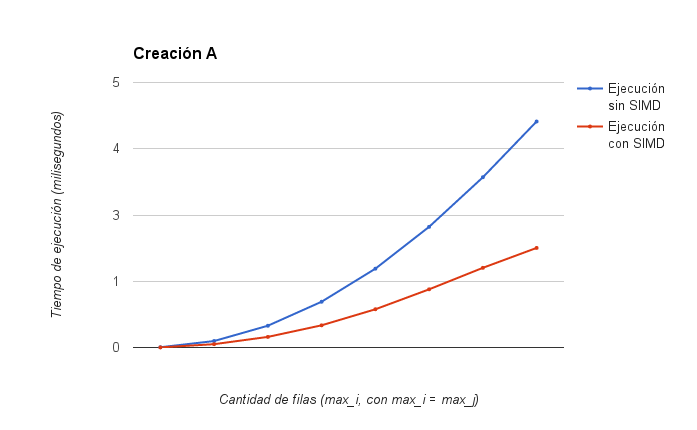
\includegraphics[scale = 0.7]{images/CreateA.png}
  \caption{Tiempo que demora la función de creación de la matriz A con y sin SIMD}
\end{figure}
\begin{figure}[!htbp]
  \centering
	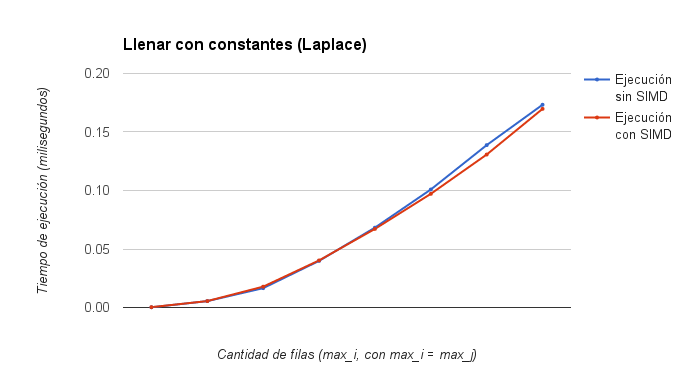
\includegraphics[scale = 0.7]{images/FillWithConstant.png}
  \caption{Tiempo que demora la función que llena una matriz con una constante con y sin SIMD}
\end{figure}
\begin{figure}[!htbp]
  \centering
	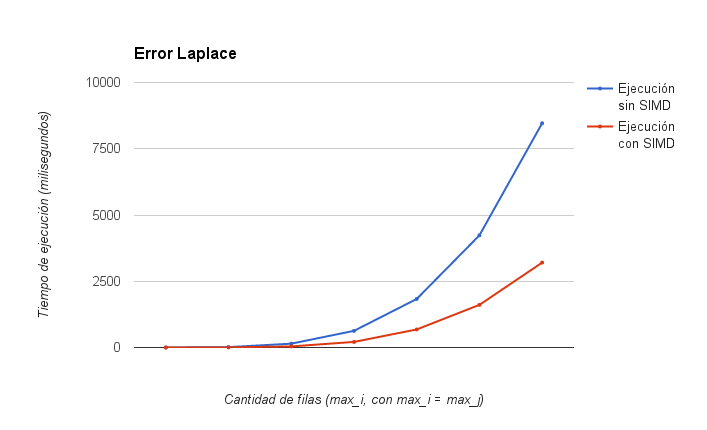
\includegraphics[scale = 0.7]{images/LaplaceError.png}
  \caption{Tiempo que demora la función de error de convergencia de Laplace con y sin SIMD}
\end{figure}
\begin{figure}[!htbp]
  \centering
	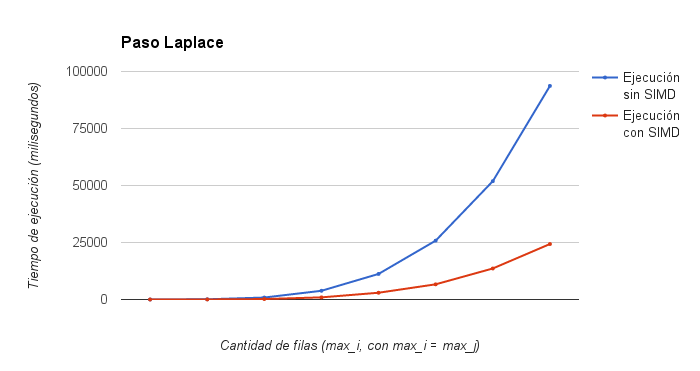
\includegraphics[scale = 0.7]{images/LaplaceStep.png}
  \caption{Tiempo que demora la función de cálculo de un paso de aproximación de Laplace con y sin SIMD}
\end{figure}
\begin{figure}[!htbp]
  \centering
	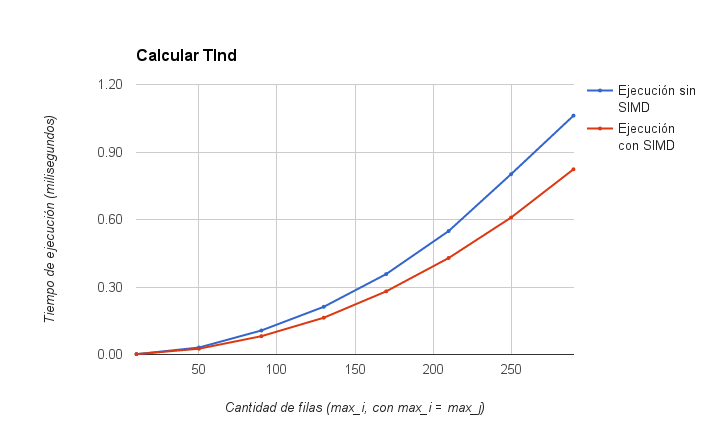
\includegraphics[scale = 0.7]{images/CalcTInd.png}
  \caption{Tiempo que demora la función de cálculo de término independiente con y sin SIMD}
\end{figure}

\begin{figure}[!htbp]
  \centering
	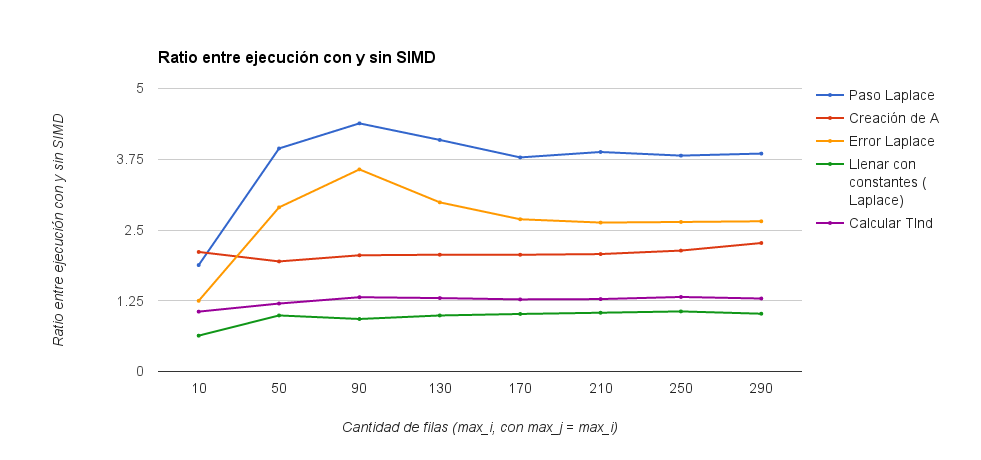
\includegraphics[scale = 0.55]{images/RatioSIMD.png}
  \caption{Razón entre el tiempo que demora cada función con y sin SIMD}
\end{figure}
\newpage
\section{Apéndice A: cálculo de temperatura en los electrodos}

Vamos a calcularlo para la pared vertical derecha de cada electrodo, los otros cálculos son análogos. El electrodo tiene 4 \textit{paredes}, pues al discretizar el tejido en una grilla el punto donde se apoya el electrodo quedará dentro de una de las casillas de la grilla.

Siendo $k$ la función definida anteriormente, sea $h = 10 \frac{W}{m^2 K}$ y $T_{aire} = 296 ^\circ K$

\begin{equation*}
\begin{aligned}
-k \frac{\partial T}{\partial x} & = h (T_{n+1}(i,j) -  T_{aire}) \\
-k \ \frac{T_{n+1}(i+1,j) - T_{n+1}(i,j)}{\Delta x} & \approx h (T_{n+1}(i,j) -  T_{aire}) \\
\frac{k}{\Delta x \cdot h} \cdot (T_{n+1}(i,j) - T_{n+1}(i+1,j)) & \approx T_{n+1}(i,j) -  T_{aire}
\end{aligned}
\end{equation*}

Utilizando el renombre $r = \frac{k}{\Delta x \cdot h}$, nos queda:

\begin{equation*}
\begin{aligned}
r \cdot (T_{n+1}(i,j) - T_{n+1}(i+1,j)) & \approx T_{n+1}(i,j) - T_{aire} \\
r \cdot T_{n+1}(i,j) - r \cdot T_{n+1}(i+1,j) & \approx T_{n+1}(i,j) - T_{aire} \\
r \cdot T_{n+1}(i,j) - T_{n+1}(i,j) & \approx r \cdot T_{n+1}(i+1,j) - T_{aire} \\
(r - 1) \cdot T_{n+1}(i,j) & \approx r \cdot T_{n+1}(i+1,j) - T_{aire} \\
T_{n+1}(i,j) & \approx \frac{r \cdot T_{n+1}(i+1,j) - T_{aire}}{r-1}
\end{aligned}
\end{equation*}

Esto mismo se puede calcular para las otras tres paredes del electrodo. En resumen, los cuatro cálculos darán como resultado lo siguiente:

\begin{equation*} \label{eq:paredes}
\begin{aligned}
T_{n+1}(i,j) & \approx \frac{r \cdot T_{n+1}(i+1,j) - T_{aire}}{r-1} \\
T_{n+1}(i,j) & \approx \frac{r \cdot T_{n+1}(i-1,j) - T_{aire}}{r-1} \\
T_{n+1}(i,j) & \approx \frac{r \cdot T_{n+1}(i,j+1) - T_{aire}}{r-1} \\
T_{n+1}(i,j) & \approx \frac{r \cdot T_{n+1}(i,j-1) - T_{aire}}{r-1}
\end{aligned}
\end{equation*}

Finalmente, aproximamos el valor de la temperatura de la casilla donde se coloca el electrodo como el promedio de la temperatura en sus cuadro bordes. Sumando las cuatro ecuaciones de (\ref{eq:paredes}):

\begin{equation*}
\begin{aligned}
4 \cdot T_{n+1}(i,j) & \approx \frac{r \cdot [T_{n+1}(i+1,j) + T_{n+1}(i-1,j) + T_{n+1}(i,j+1) + T_{n+1}(i,j-1)] - 4 \cdot T_{aire}}{r-1} \\
T_{n+1}(i,j) & \approx \frac{r}{4 \cdot (r-1)} \cdot \big(T_{n+1}(i+1,j) + T_{n+1}(i-1,j) + T_{n+1}(i,j+1) + T_{n+1}(i,j-1)\big) - \frac{T_{aire}}{r-1}
\end{aligned}
\end{equation*}

\newpage
\section{Apéndice B: cálculo del potencial eléctrico}

El potencial eléctrico es un campo escalar definido como la solución 
de la ecuación de Laplace ($\delta \varphi = 0$) dados dos puntos 
fijos (ánodo y ćatodo) y condición de borde de flujo cero.\\
La discretización de la ecuación $\delta \varphi = 0$ es conocida y 
corresponde a que una posición es el promedio de sus vecinos. 
Es decir, $$\varphi(i, j) = \frac{\varphi(i-1, j) + \varphi(i+1, j) + \varphi(i, j-1) + \varphi(i, j+1)}{4}$$
Por otro lado, la condición de borde es la misma que en el caso de 
la ecuación de calor, por lo que las fórmulas de las discretizaciones 
en los puntos del borde son análogas y equivalen a:
\begin{equation*}
\begin{aligned}
\varphi(0,j) & = \varphi(1,j) \\ 
\varphi(i,0) & = \varphi(i,1) \\
\varphi(i,max_j) & = \varphi(i,max_j-1) \\ 
\varphi(max_i,j) & = \varphi(max_i-1,j)
\end{aligned}
\end{equation*}
Para obtener una solución aproximada del sistema, iteramos reemplazando el potencial actual de cada posición por el promedio de sus vecinos hasta que estos valores converjan.

\end{document}
